\documentclass[nooutcomes,space,handout]{ximera}
%\documentclass[space,handout,nooutcomes]{ximera}

% For preamble materials

\usepackage{pgf,tikz}
\usepackage{mathrsfs}
\usetikzlibrary{arrows}
\usepackage{framed}
\usepackage{amsmath}
\pgfplotsset{compat=1.17}

\def\fixnote#1{\begin{framed}{\textcolor{red}{Fix note: #1}}\end{framed}}  % Allows insertion of red notes about needed edits
%\def\fixnote#1{}

\def\detail#1{{\textcolor{blue}{Detail: #1}}}   

\pdfOnly{\renewenvironment{image}[1][]{\begin{center}}{\end{center}}}

\graphicspath{
  {./}
  {chapter1/}
  {chapter2/}
  {chapter4/}
  {proofs/}
  {graphics/}
  {../graphics/}
}

\newenvironment{sectionOutcomes}{}{}


%%% This set of code is all of our user defined commands
\newcommand{\bysame}{\mbox{\rule{3em}{.4pt}}\,}
\newcommand{\N}{\mathbb N}
\newcommand{\C}{\mathbb C}
\newcommand{\W}{\mathbb W}
\newcommand{\Z}{\mathbb Z}
\newcommand{\Q}{\mathbb Q}
\newcommand{\R}{\mathbb R}
\newcommand{\A}{\mathbb A}
\newcommand{\D}{\mathcal D}
\newcommand{\F}{\mathcal F}
\newcommand{\ph}{\varphi}
\newcommand{\ep}{\varepsilon}
\newcommand{\aph}{\alpha}
\newcommand{\QM}{\begin{center}{\huge\textbf{?}}\end{center}}

\renewcommand{\le}{\leqslant}
\renewcommand{\ge}{\geqslant}
\renewcommand{\a}{\wedge}
\renewcommand{\v}{\vee}
\renewcommand{\l}{\ell}
\newcommand{\mat}{\mathsf}
\renewcommand{\vec}{\mathbf}
\renewcommand{\subset}{\subseteq}
\renewcommand{\supset}{\supseteq}
%\renewcommand{\emptyset}{\varnothing}
%\newcommand{\xto}{\xrightarrow}
%\renewcommand{\qedsymbol}{$\blacksquare$}
%\newcommand{\bibname}{References and Further Reading}
%\renewcommand{\bar}{\protect\overline}
%\renewcommand{\hat}{\protect\widehat}
%\renewcommand{\tilde}{\widetilde}
%\newcommand{\tri}{\triangle}
%\newcommand{\minipad}{\vspace{1ex}}
%\newcommand{\leftexp}[2]{{\vphantom{#2}}^{#1}{#2}}

%% More user defined commands
\renewcommand{\epsilon}{\varepsilon}
\renewcommand{\theta}{\vartheta} %% only for kmath
\renewcommand{\l}{\ell}
\renewcommand{\d}{\, d}
\newcommand{\ddx}{\frac{d}{dx}}
\newcommand{\dydx}{\frac{dy}{dx}}


\usepackage{bigstrut}


\title{Proof by Picture 1}
\author{Bart Snapp and Brad Findell}
\begin{document}
\begin{abstract}
Short-answer proofs about triangle area. 
\end{abstract}
\maketitle

% No change?

\begin{problem}
Explain how the following picture ``proves'' that
  the area of a right triangle is half the base times the height.
\begin{image}
%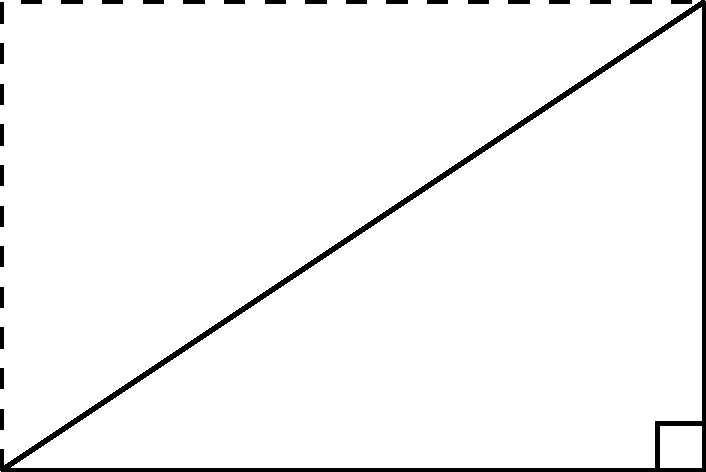
\includegraphics{pbpAreaRight.png}
\definecolor{qqwuqq}{rgb}{0.,0.392,0.}
\begin{tikzpicture}%[line cap=round,line join=round,>=triangle 45,x=1.0cm,y=1.0cm]
\draw[line width=0.8pt,color=qqwuqq,fill=qqwuqq,fill opacity=0.10] (0.28,0.) -- (0.28,0.28) -- (0.,0.28) -- (0.,0.) -- cycle; 
\draw [line width=0.8pt] (0.,3.)-- (0.,0.) -- (4.,0.) -- cycle;
\draw [line width=0.8pt,dash pattern=on 2pt off 2pt] (0.,3.)-- (4.,3.) -- (4.,0.);
\draw [color=white] (-4.,0.) circle (0.2pt);
\draw [color=white] (8.,0.) circle (0.2pt);
\end{tikzpicture}
\end{image}
\begin{freeResponse}
\end{freeResponse}

\begin{problem}
The area of the rectangle is base times height.  The rectangle is made up of two congruent right triangles.  Because congruent triangles have the same area, the area of each right triangle is \wordChoice{\choice{equal to}\choice[correct]{half}\choice{double}} the area of the rectangle.  
\end{problem}

\end{problem}

\begin{problem}
Suppose you know that the area of a \textbf{right} triangle is
  half the base times the height. Explain how the following picture
  ``proves'' that the area of \textbf{every} triangle is half the base times the
  height.
\begin{image}
%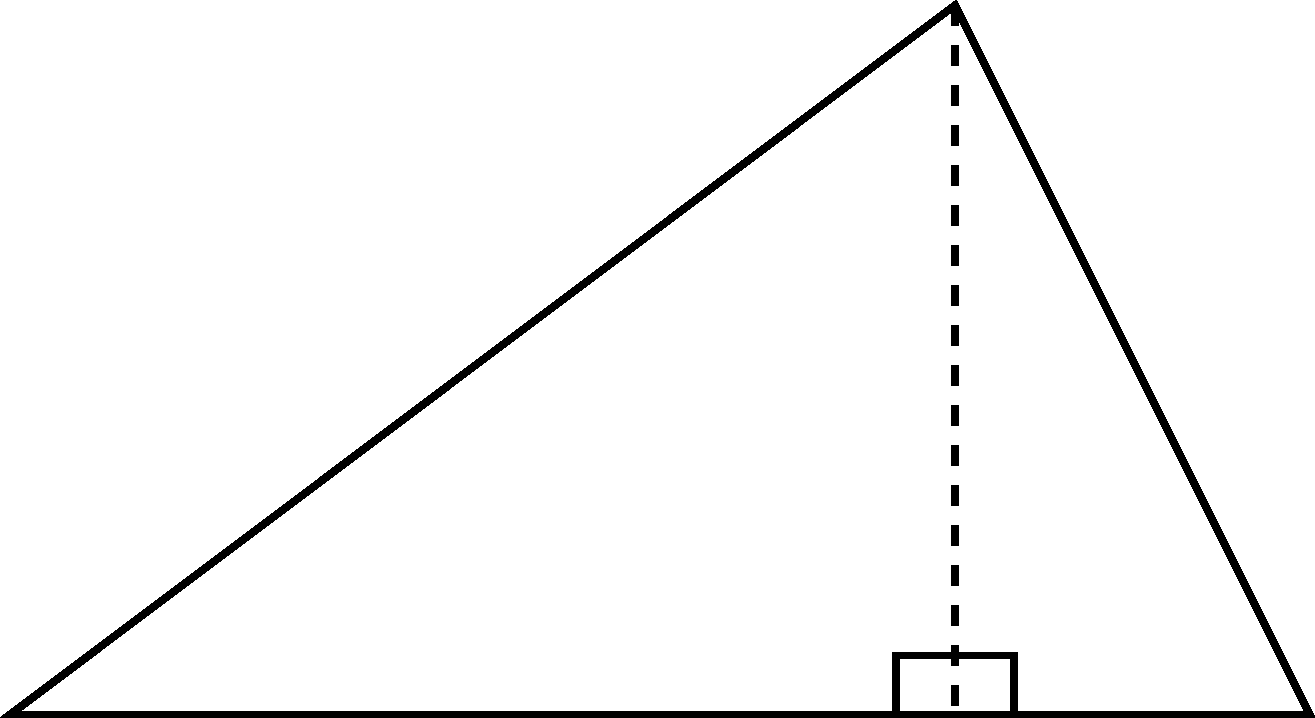
\includegraphics{pbpDisTri.png}
\definecolor{qqwuqq}{rgb}{0.,0.392,0.}
\begin{tikzpicture}[line cap=round,line join=round,>=triangle 45,x=1.0cm,y=1.0cm]
\draw[line width=0.8pt,color=qqwuqq,fill=qqwuqq,fill opacity=0.1] (3.,0.1954) -- (2.8046,0.1954) -- (2.8046,0.) -- (3.,0.) -- cycle; 
\draw[line width=0.8pt,color=qqwuqq,fill=qqwuqq,fill opacity=0.1] (3.1954,0.) -- (3.1954,0.1954) -- (3.,0.1954) -- (3.,0.) -- cycle; 
\draw [line width=0.8pt] (0.,0.)-- (3.,1.8);
\draw [line width=0.8pt] (3.,1.8)-- (4.5,0.);
\draw [line width=0.8pt] (4.5,0.)-- (0.,0.);
\draw [line width=0.8pt,dash pattern=on 2pt off 2pt] (3.,0.)-- (3.,1.8);
\draw [color=white] (-4.,0.) circle (0.1pt);
\draw [color=white] (8.,0.) circle (0.1pt);
\end{tikzpicture}
\end{image}

\begin{freeResponse}
\end{freeResponse}

\begin{problem}
Surround the triangle with a rectangle as shown.    
\begin{image}
%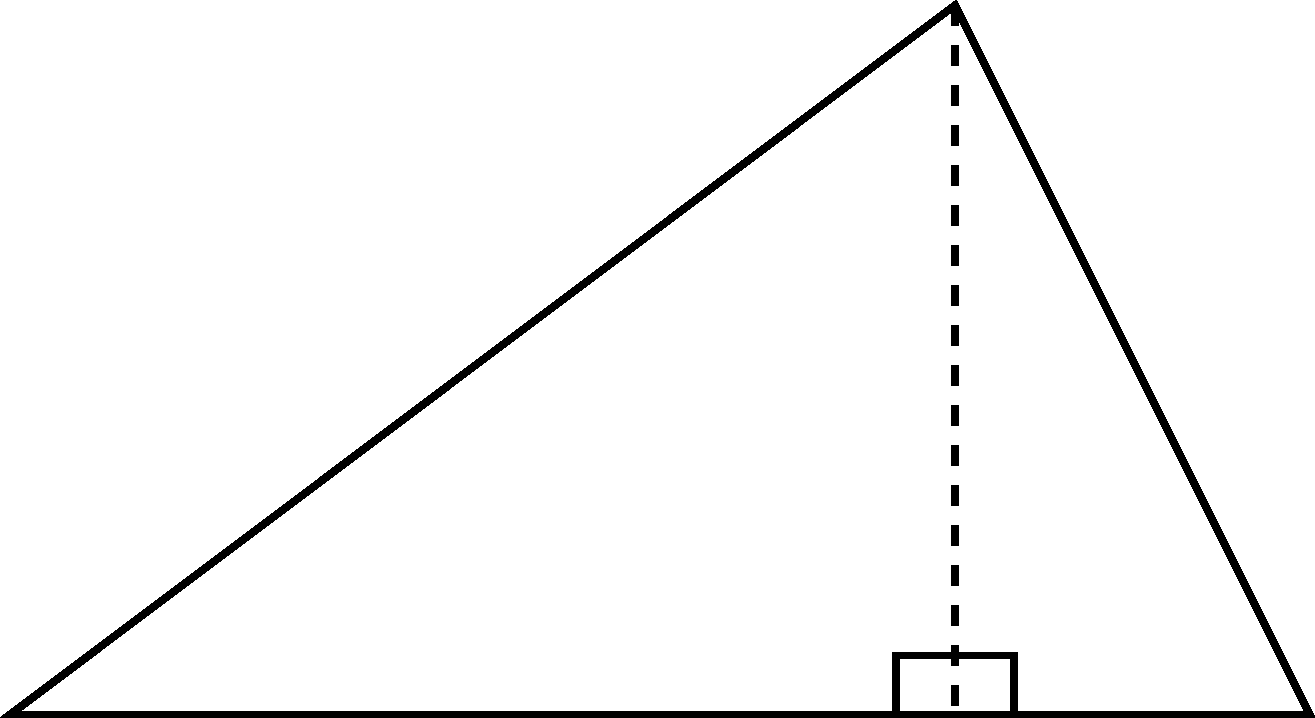
\includegraphics{pbpDisTri.png}
\definecolor{qqwuqq}{rgb}{0.,0.392,0.}
\begin{tikzpicture}[line cap=round,line join=round,>=triangle 45,x=1.0cm,y=1.0cm]
\draw[line width=0.8pt,color=qqwuqq,fill=qqwuqq,fill opacity=0.1] (3.,0.1954) -- (2.8046,0.1954) -- (2.8046,0.) -- (3.,0.) -- cycle; 
\draw[line width=0.8pt,color=qqwuqq,fill=qqwuqq,fill opacity=0.1] (3.1954,0.) -- (3.1954,0.1954) -- (3.,0.1954) -- (3.,0.) -- cycle; 
\draw [line width=0.8pt] (0.,0.)-- (3.,1.8) -- (4.5,0.) -- cycle;
\draw [line width=0.8pt,dash pattern=on 2pt off 2pt] (3.,0.)-- (3.,1.8);
\draw [line width=0.8pt,dash pattern=on 2pt off 2pt] (0.,0.)-- (0.,1.8) -- (4.5,1.8)-- (4.5,0.);
\draw [color=white] (-4.,0.) circle (0.1pt);
\draw [color=white] (8.,0.) circle (0.1pt);
\end{tikzpicture}
\end{image}
Then the solid triangle is again $\answer[format=string]{half}$ the rectangle, and they have the same base and the same height.
\end{problem}

\begin{problem}
The whole triangle is made up of two right triangles.  Call the bases of the small right triangles $b_1$ and $b_2$, and call the base of the large (combined) triangle $b$.  
\begin{image}
%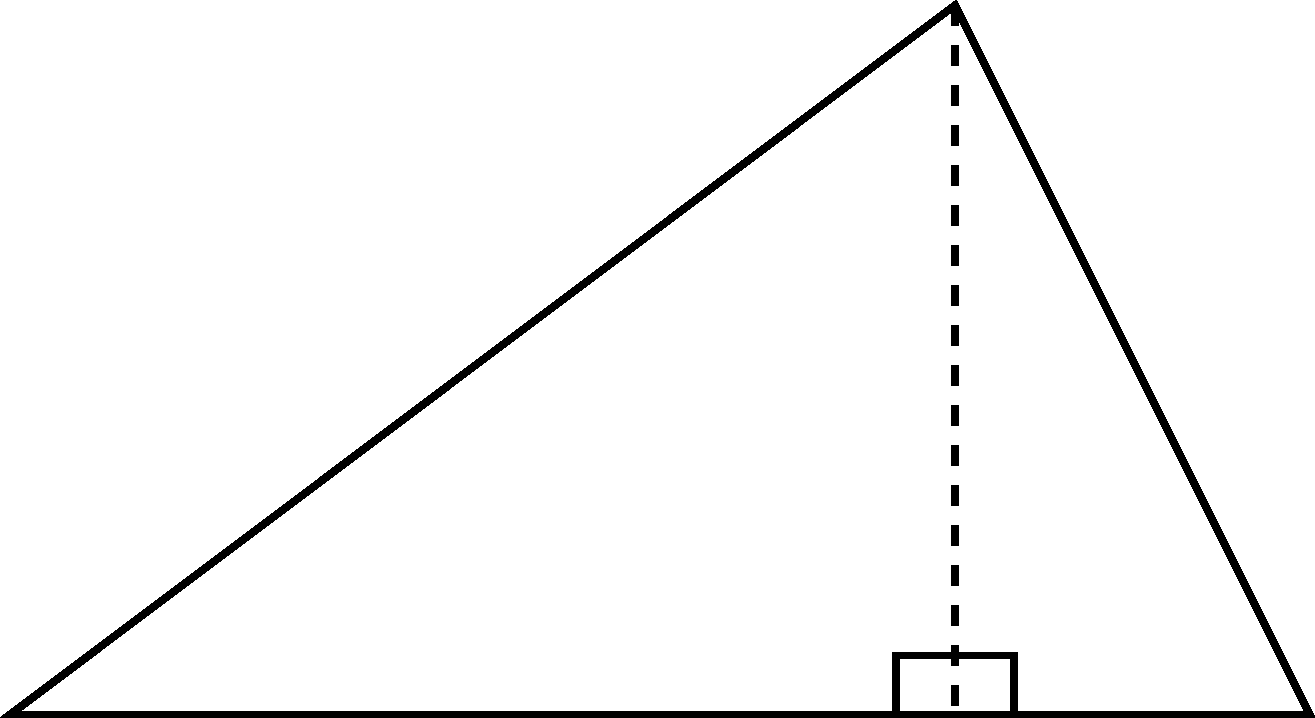
\includegraphics{pbpDisTri.png}
\definecolor{qqwuqq}{rgb}{0.,0.392,0.}
\begin{tikzpicture}%[line cap=round,line join=round,>=triangle 45,x=1.0cm,y=1.0cm]
\draw[line width=0.8pt,color=qqwuqq,fill=qqwuqq,fill opacity=0.1] (3.,0.1954) -- (2.8046,0.1954) -- (2.8046,0.) -- (3.,0.) -- cycle; 
\draw[line width=0.8pt,color=qqwuqq,fill=qqwuqq,fill opacity=0.1] (3.1954,0.) -- (3.1954,0.1954) -- (3.,0.1954) -- (3.,0.) -- cycle; 
\draw [line width=0.8pt] (0.,0.)-- (3.,1.8) -- (4.5,0.) -- cycle;
\draw [line width=0.8pt,dash pattern=on 2pt off 2pt] (3.,0.)-- (3.,1.8);
\draw [color=white] (-4.,0.) circle (0.1pt);
\draw [color=white] (8.,0.) circle (0.1pt);
\draw (1.6,-0.2) node {$b_1$};
\draw (3.8,-0.2) node {$b_2$};
\draw (2.8,1.0) node {$h$};
\end{tikzpicture}
\end{image}
Then $b=b_1+b_2$, and the three triangles all have the same height, $\answer{h}$.   The area of the whole triangle is the sum of the areas of the two right triangles:  
\[
\mathrm{Area} =  \frac{hb_1}{2}+ \frac{hb_2}{2}= \frac{h(b_1 + b_2)}{2} = \answer{bh/2}
\]
because $b=b_1+b_2$.
\end{problem}

\end{problem}

\begin{problem}
Now suppose that a student, say \textit{Geometry Giorgio} attempts to
solve a similar problem. Again knowing that the area of a right
triangle is half the base times the height, he draws the following
picture:
\begin{image}
%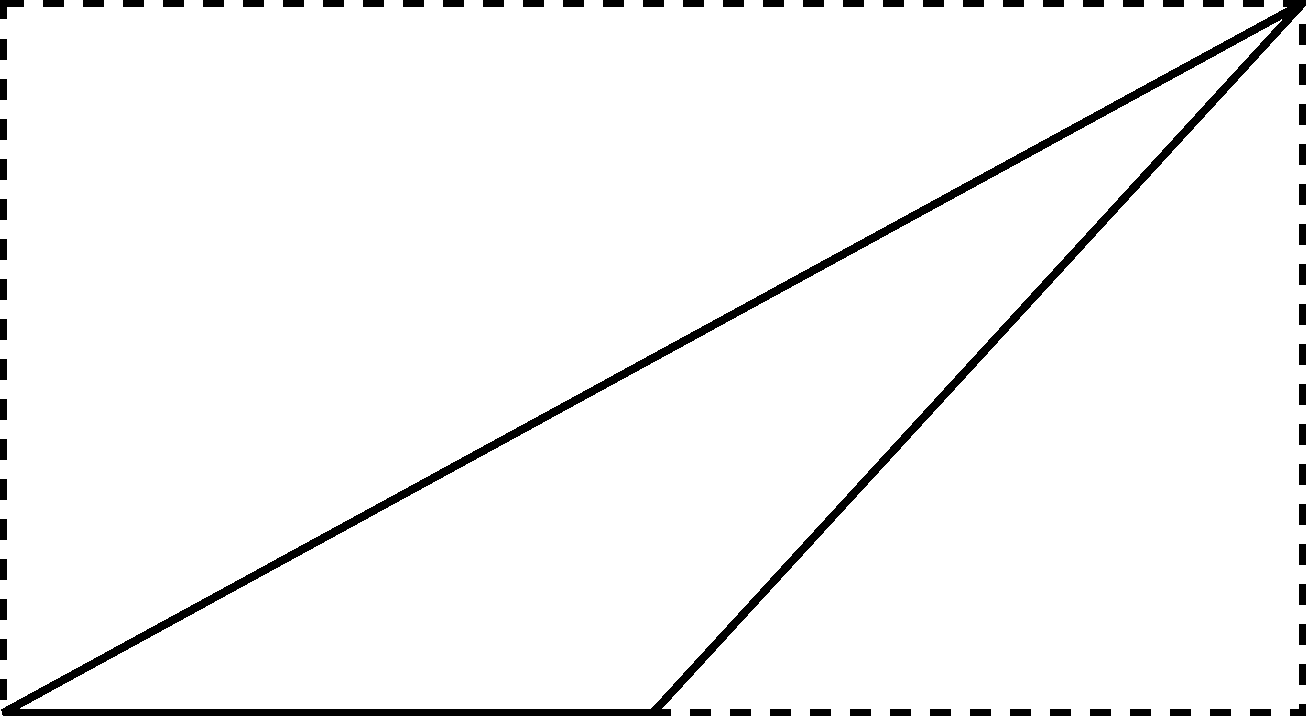
\includegraphics{pbpDisTriGio.png}
\begin{tikzpicture}%[line cap=round,line join=round,>=triangle 45,x=1.0cm,y=1.0cm]
\draw [line width=0.8pt,dash pattern=on 2pt off 2pt] (0.,0.)-- (0.,2.5) -- (5.,2.5) -- (5.,0.) -- (2.,0.);
\draw [line width=0.8pt] (0.,0.)-- (2.,0.) -- (5.,2.5) -- cycle;
\draw [color=white] (-4.,0.) circle (0.2pt);
\draw [color=white] (8.,0.) circle (0.2pt);
\end{tikzpicture}
\end{image}
\textit{Geometry Giorgio} states that the diagonal line cuts the
rectangle in half, and thus the area of the triangle is half the base
times the height. Is this correct reasoning? 

%If so, give a complete
%explanation. If not, give correct reasoning based on \textit{Geometry
%  Giorgio's} picture.

Response: The area of the solid triangle is
\wordChoice{\choice{greater than}\choice{equal to}\choice[correct]{less than}} half the area of the rectangle.  Furthermore, the rectangle 
\wordChoice{\choice[correct]{does not have}\choice{has}} the same base as the triangle, so ``half the base times height'' is 
\wordChoice{\choice[correct]{unclear}\choice{correct}\choice{incorrect}}.  

\begin{problem}
To get a better sense of Giorgio's triangle, try some numbers.  
\begin{image}
\begin{tikzpicture}%[line cap=round,line join=round,>=triangle 45,x=1.0cm,y=1.0cm]
\draw [line width=0.8pt,dash pattern=on 2pt off 2pt] (0.,0.)-- (0.,2.5) -- (5.,2.5) -- (5.,0.) -- (2.,0.);
\draw [line width=0.8pt] (0.,0.)-- (2.,0.) -- (5.,2.5) -- cycle;
\draw (1.1,-0.2) node {$4$};
\draw (3.5,-0.2) node {$6$};
\draw (5.2,1.3) node {$5$};
\draw [color=white] (-4.,0.) circle (0.2pt);
\draw [color=white] (8.,0.) circle (0.2pt);
\end{tikzpicture}
\end{image}
Find the area of this triangle (which is much less than half the rectangle).  

\begin{align*}
\begin{minipage}{2cm}\center{\textrm{Area of solid triangle}}\end{minipage}  &= 
            \begin{minipage}{2cm}\center{\textrm{Area of rectangle}}\end{minipage} &-& 
            \begin{minipage}{2cm}\center{\textrm{Area of large right triangle}}\end{minipage} &-& 
            \begin{minipage}{2cm}\center{\textrm{Area of small right triangle}}\end{minipage} \\
      &= \answer{50} &-& \answer{25} &-& \answer{15} \\
      &= \answer{10}
\end{align*}


\begin{problem}
Maybe a grid will help.    
\begin{image}
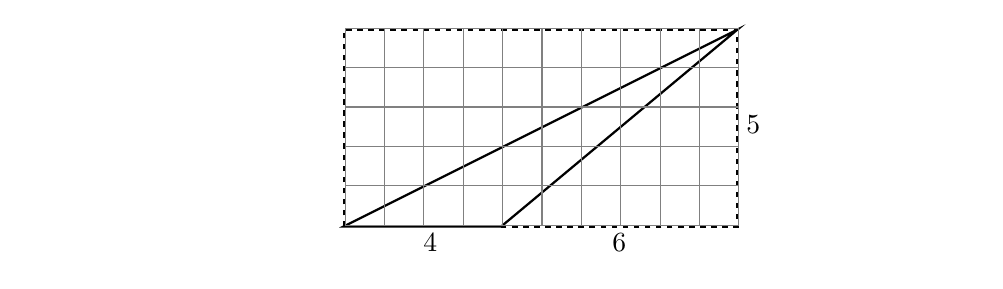
\begin{tikzpicture}%[line cap=round,line join=round,>=triangle 45,x=1.0cm,y=1.0cm]
\draw [line width=0.8pt,dash pattern=on 2pt off 2pt] (0.,0.)-- (0.,2.5) -- (5.,2.5) -- (5.,0.) -- (2.,0.);
\draw [line width=0.8pt] (0.,0.)-- (2.,0.) -- (5.,2.5) -- cycle;
\draw (1.1,-0.2) node {$4$};
\draw (3.5,-0.2) node {$6$};
\draw (5.2,1.3) node {$5$};
%% Dot grid
%\foreach \x in {0,0.5,...,5} {
%    \foreach \y in {0,0.5,...,2.5} {
%        \fill[color=gray] (\x,\y) circle (0.04);
%    }
% }
\draw[step=0.5,gray,thin,xshift=0.5,yshift=0.5] (0.0,0.0) grid (5.0,2.5);
\draw [color=white] (-4.,0.) circle (0.2pt);
\draw [color=white] (8.,0.) circle (0.2pt);
\end{tikzpicture}
\end{image}
\end{problem}

\end{problem}

\begin{problem}
The following picture generalizes this approach.   
\begin{image}
\begin{tikzpicture}%[line cap=round,line join=round,>=triangle 45,x=1.0cm,y=1.0cm]
\draw [line width=0.8pt,dash pattern=on 2pt off 2pt] (0.,0.)-- (0.,2.5) -- (5.,2.5) -- (5.,0.) -- (2.,0.);
\draw [line width=0.8pt] (0.,0.)-- (2.,0.) -- (5.,2.5) -- cycle;
\draw (1.1,-0.2) node {$b$};
\draw (3.5,-0.2) node {$x$};
\draw (5.2,1.3) node {$h$};
\draw [color=white] (-4.,0.) circle (0.2pt);
\draw [color=white] (8.,0.) circle (0.2pt);
\end{tikzpicture}
\end{image}

One way to compute the area of the solid triangle is to (1) compute the area right triangle that is the lower half of the rectangle (with base $b+x$) and then (2) subtract the area of the small right triangle (with base $x$): 
\[
\mathrm{area} =  \answer{\frac{h(b+x)}{2}} - \answer{\frac{hx}{2}}= \frac{hb+hx}{2} - \frac{hx}{2}
= \left(\frac{hb}{2} + \frac{hx}{2}\right) - \frac{hx}{2} = \answer{\frac{hb}{2}}
\]
\end{problem}
\end{problem}

\end{document}
